\section{Hidden Markov Models}
\label{sec:hmm}
\glspl{hmm} are one of the most widely used and best known variants of probabilistic finite automata~\cite{pautomacTR, Rabiner89hmm}. The theoretical basis for \glspl{hmm} and associated methods and algorithms were first described in a series of works by L. E. Baum~et~al.~\cite{baum1966, baum1967, baum1968, baum1970, baum1972}.

One can view an \gls{hmm} as an extension of a standard Markov chain. A Markov chain based model has the property that every observed symbol corresponds directly to an associated state of the model. This property is too restrictive for numerous problems. \glspl{hmm} therefore introduce the concept of hidden (unobservable) states with a probability distribution over the observable symbols. The generated symbol thus becomes a probabilistic function of the current hidden state. This extension allows application of \glspl{hmm} to a much larger variety of problems, however also poses new complications, such as increased complexity of evaluation of probability of a given signal (sequence of observable symbols), determining the optimal sequence of hidden states for a given signal or estimation of parameters for the model~\cite{Rabiner89hmm}.

To better illustrate the mechanics behind the \gls{hmm} we provide a simple example. Consider a lottery game with several urns filled with balls of different colours. Every urn may hold different number of balls of a certain colour, or may not even contain balls of some colours at all. In every turn an unbiased arbiter selects one urn randomly (but possibly abiding to some rules given by the urn selected previously) and takes out a random ball out of the selected urn. You are then shown the colour of the ball, not however, from which urn it was taken. The ball is then returned to the appropriate urn and the game continues so forth your goal being to predict the colours that come next. In this simple case, you can observe a sequence of symbols - colours generated by what can be viewed as an \gls{hmm}, where the urns are the hidden states and the observable symbol probability distribution for every urn (state) is given by the colours of the balls inside.

More formally, a finite discrete \acrlong{hmm} with $n \in \mathbb{N}$ (hidden) states $S = \{S_1, S_2, ..., S_n\}$ over an alphabet of $m \in \mathbb{N}$ observable symbols $\Sigma=\{\sigma_1, \sigma_2, ..., \sigma_m\}$ is a tuple: $$\lambda = (\mathbf{A}, \mathbf{B}, \boldsymbol{\pi})$$
Where:
\begin{itemize}
	\item[$\mathbf{A}$] is an $n$ times $n$ square matrix such that an element of the matrix ${a_{ij} \in [0, 1]}$ represents the transition probability from state $S_i$ to state $S_j$. Naturally this implies ${\forall i \in \{1, 2, ..., n\}: \sum_{j=1}^n{a_{ij}} = 1}$.
	\item[$\mathbf{B}$] is an $n$ times $m$ matrix such that an element of the matrix ${b_{ij} \in [0, 1]}$ represents the probability of outputting symbol $\sigma_j$ in state $S_i$. Naturally this implies ${\forall i \in \{1, 2, ..., n\}: \sum_{j=1}^m{b_{ij}} = 1}$.
	\item[$\boldsymbol{\pi}$] is a vector of $n$ variables, ${\boldsymbol{\pi}=(\pi_1, ..., \pi_n) \in [0, 1]^n}$. Where the value $\pi_i$ represents the probability of state $S_i$ being the initial state. Naturally this implies ${\sum_{i=1}^n{\pi_i} = 1}$
\end{itemize}

Such an \gls{hmm} can be used to generate a sequence of observable symbols (signal): $$\mathbf{O} = (o_1, ..., o_T)$$
Where ${\forall t \in \{1, ..., T\}: o_t \in \Sigma}$, $o_t$ is the symbol observed at time $t$ and $T$ is the number of discrete time steps during the observation (number of observed symbols).

Similarly, we denote a sequence of hidden states of the hidden Markov model as: $$\mathbf{Q} = (q_1, ..., q_T)$$
Where ${\forall t \in \{1, ..., T\}: q_t \in S}$, $q_t$ is the state of the model at time $t$ and $T$ is the number of visited states.
We define the probability of the hidden state sequence (walk) $\mathbf{Q}$ given the model $\lambda$ as:
$$P(\mathbf{Q}|\lambda) = \pi_{q_1}a_{q_1q_2}...a_{q_{T-1}q_T}$$

Any signal $\mathbf{O}$ generated by the \gls{hmm} has a corresponding sequence of hidden states $\mathbf{Q}$ the model visited during the generation of the same length. This sequence is typically unknown for modeled real world signals and generally numerous different hidden state sequences may generate the observed signal with different probabilities. We denote the probability of model $\lambda$ producing the observation sequence $\mathbf{O}$ by hidden state sequence $\mathbf{Q}$ as:
$$P(\mathbf{O}|\mathbf{Q},\lambda) = b_{q_1}(o_1)b_{q_2}(o_2)b_{q_T}(o_T)$$

In the above probability definitions we use more lenient notation for simplicity. As the use of this notation is preserved throughout the following sections alongside the notation from definition of the \gls{hmm}. We define it formally for clarity:
\begin{itemize}
	\item[] $a_{S_iS_j}$ where $S_i, S_j\in S$ is used to refer to the value of $a_{ij}$.
	\item[] $\pi_{S_i}$ where $S_i\in S$ is used to refer to the value of $\pi_i$.
	\item[] $b_{S_i}(\sigma_j)$ where $S_i\in S$ and $\sigma_j\in \Sigma$ is used to refer to the value of $b_{ij}$.
\end{itemize}

Furthermore let us define the set of all possible walks through hidden state space of model $\lambda$ of length $T$ as $\mathcal{Q}_\lambda^T$. Thus the probability of model $\lambda$ generating the signal $\mathbf{O}$ can be easily defined as a sum of probabilities of generating the given signal through all hidden state walks weighted by probabilities of the particular hidden state walks: 

\begin{align*}
P(\mathbf{O}|\lambda)&=\sum_{\mathbf{Q}\in\mathcal{Q}^T_\lambda}{P(\mathbf{O}|\mathbf{Q},\lambda)P(\mathbf{Q}|\lambda)}\\
&=\sum_{\mathbf{Q}\in\mathcal{Q}^T_\lambda}{\pi_{q_1}b_{q_1}(o_1)a_{q_1q_2}b_{q_2}(o_2)...a_{q_{T-1}q_T}b_{q_T}(o_T)}
\end{align*}

It should be noted that the \gls{hmm} defined here is finite in the sense of both $n$ and $m$ being finite numbers. An extension to the model allowing infinite number of states, symbols or both is rather straightforward, however we will not be needing this extension for the purposes of this publication and thus it will be omitted.

\subsection{Hidden Markov Model Evaluation}
It is meaningful and desirable to evaluate a model once constructed and learned. Such evaluation is usually done by computing the probability of the model producing a certain observation sequence. Therefore for a model $\lambda = (\mathbf{A}, \mathbf{B}, \boldsymbol{\pi})$ and a (test) sequence $\mathbf{O}$, we want to learn $P(\mathbf{O}|\lambda)$. Going by the definition one arrives at a summation over all possible walks through hidden state space of model $\lambda$ of length $T$. It is simple to see that, with the presumption that the model is unrestricted (i.e., matrix $\mathbf{A}$ is dense), there is exponentially many of such walks in terms of their length $T$ ($|\mathcal{Q}_\lambda^T|\in\mathcal{O}(N^T)$). Computing the given summation and thereafter computing $P(\mathbf{O}|\lambda)$ by definition is computationally infeasible.

Luckily, an iterative dynamic programming approach exists that can help us compute the coveted probability, called the \gls{fb_algorithm}~\cite{baum1967, baum1968}. The \gls{fb_algorithm} is composed of computing two separate sets of variables (forward and backward), both of which can be used to compute the probability $P(\mathbf{O}|\lambda)$.

The forward variable $\alpha_t(i)$, formally defined as: $$\alpha_t(i)=P((o_1, ..., o_t), q_t=S_i|\lambda)$$ describes the probability that we observe the first $t$ symbols of the given signal and end in the state $S_i$ at the time $t$ given the model $\lambda$.

The forward variable can be computed iteratively as:
\begin{align*}
\forall i\in \{1, ..., n\}&: \alpha_1(i)=\pi_ib_{S_i}(o_1)\\
\forall i\in \{1, ..., n\}, t\in\{2, ..., T\}&: \alpha_t(i) = \sum_{j=1}^n{(\alpha_{t-1}(j)a_{ji})}b_{S_i}(o_t)
\end{align*}

It is easy to see that the probability of an observable sequence $\mathbf{O}$ can be obtained by summing through the forward variables at time $T$ for all of the hidden states:
\begin{align*}
P(\mathbf{O}|\lambda) &= \sum_{i=1}^n{P(\mathbf{O}, q_T=S_i|\lambda)}\\
&= \sum_{i=1}^n{\alpha_T(i)}
\end{align*}

Analogically, the backward variable $\beta_t(i)$, formally defined as: $$\beta_t(i)=P((o_{t+1}, ..., o_T)| q_t=S_i, \lambda)$$ describes the probability that we observe the last $(T-t+1)$ symbols of signal $\mathbf{O}$ given we start at state $S_i$ at the time $t$ and the model $\lambda$.

Again, computing the backward variable is possible iteratively:
\begin{align*}
\forall i\in \{1, ..., n\}&:\beta_T(i)=1\\
\forall i\in\{1, ..., n\}, t\in\{1, ..., T-1\}&:\beta_t(i)=\sum_{j=1}^n{(a_{ij}b_{S_j}(o_{t+1})\beta_{t+1}(j))}
\end{align*}

Once again we straightforwardly obtain a simple way of computing $P(\mathbf{O}|\lambda)$:
\begin{align*}
P(\mathbf{O}|\lambda) &= \sum_{i=1}^n{P(\mathbf{O}|q_1=S_i, \lambda)}\\
&= \sum_{i=1}^n{\beta_1(i)}
\end{align*}

After a careful observation one can see that both approaches, using forward or backward variables, give as an efficient way to compute $P(\mathbf{O}|\lambda)$ in complexity $\mathcal{O}(Tn^2)$~\cite{Rabiner89hmm}.

\subsection{Optimal Hidden State Sequence}

It may be useful to determine the hidden state sequence the model used to generate a given observable signal. Which hidden state sequence is optimal is heavily dependent on the optimality criterion. Multiple optimality criteria exist and are meaningful to use for some applications. The most widely used optimality criterion maximises the probability of the whole walk through the hidden state space given the model $\lambda$ and the observable sequence $\mathbf{O}$~\cite{Rabiner89hmm}:
$$\max_{\mathbf{Q}\in\mathcal{Q}_T^\lambda}(P(\mathbf{Q}|\mathbf{O}, \lambda))$$

An algorithmic solution exists for optimisation of maximisation of $P(\mathbf{O}, \mathbf{Q}|\lambda)$, equivalent to the above expression, based on dynamic programing methods, called \gls{viterbi}~\cite{Viterbi1967, Forney1973}. The algorithm iteratively computes the best single state path score for the first $t$ symbols of the observed sequence. We denote this score for state $i$ and time $t$ as $\delta_t(i)$:
$$\delta_t(i) = \max_{q_1, ..., q_{t-1}}(P((o_1, ..., o_t), (q_1, ..., q_{t-1}), q_t=S_i|\lambda))$$

The \gls{viterbi} is briefly illustrated by the following pseudocode:
\begin{lstlisting}[mathescape=true]
real, int[] Viterbi (int n, int T, real[,] A,
 real[,] B, real[] $\pi$, int[] O) begin
   real[,] $\delta$ := new real[T,n] //$\delta$[t,i] = $\delta_t(i)$
   int[,] $\psi$ := new int[T,n] //For backtracking
   real p := 0.0 //Best score
   int[] q := new int[T] //Optimal sequence
   
   //Initialisation
   for int i := 1 to n do begin
      $\delta$[1,i] := $\pi$[i]B[i,O[1]]
      $\psi$[1,i] := 0
   end
   
   //Iteration
   for int t := 2 to T do begin
      for int j := 1 to n do begin
         $\delta$[t,j] := 0
         for int i := 1 to n do begin //Maximum over i
            if $\delta$[t,j] < $\delta$[(t - 1),i]A[i,j]B[j,O[t]] then
             do begin
               $\delta$[t,j] := $\delta$[(t - 1),i]A[i,j]B[j,O[t]]
               $\psi$[t,j] := i
            end
         end
      end
   end
   
   //Termination
   for int i := 1 to n do begin //Maximum over i
      if p < $\delta$[T,i] then do begin
         p := $\delta$[T,i]
         q[T] := i
      end
   end
   
   //Backtracking
   for int t := (T - 1) downto 1 do
      q[t] := $\psi$[(t + 1), q[t + 1]]

   return p, q;
end
\end{lstlisting}

\subsection{Estimating Model Parameters}
\label{sec:baum-welch}
There is no analytical solution known for finding model parameters $\mathbf{A}$, $\mathbf{B}$ and $\boldsymbol{\pi}$ maximising the probability of a given observable sequence. In fact, no optimal way to estimate the parameters for \glspl{hmm} exists. However, an iterative method, the \gls{baum-welch}~\cite{baum1970}, can be used to derive $\lambda = (\mathbf{A}, \mathbf{B}, \boldsymbol{\pi})$ such that $P(\mathbf{O}|\lambda)$ is locally maximised for a given signal $\mathbf{O}$. The \gls{baum-welch} has been shown to be equivalent to the \gls{em} method for \glspl{hmm}~\cite{Dempster1977, wu1983}.

In this section we present a simple iterative approach to estimation of \gls{hmm} parameters based primarily on the \gls{baum-welch}. This approach works for a single observable symbol sequence, however the \gls{baum-welch} can be extended to account for train data composed of multitude of signals~\cite{Rabiner89hmm, levinson1983, li2000}.

We first define a couple of auxiliary variables to simplify the consequent constructs:

\begin{align*}
\forall t\in\{1,...,T-1\},\forall i,j\in \{1,...,n\}: \xi_t(i,j) &= P(q_t =S_i, q_{t+1}=S_j|\mathbf{O},\lambda)\\
&= \frac{\alpha_t(i)a_{ij}b_{S_j}(o_{t+1})\beta_{t+1}(j)}{\sum_{k=1}^n\sum_{l=1}^n(\alpha_t(k)a_{kl}b_{S_l}(o_{t+1})\beta_{t+1}(l))}\\
\\
\forall t\in\{1,...,T-1\},\forall i\in\{1,...,n\}: \gamma_t(i) &=P(q_t=S_i|\mathbf{O},\lambda)\\
&=\sum_{j=1}^n\xi_t(i,j)\\
\forall i\in\{1,...,n\}: \gamma_T(i) &= P(q_T=S_i|\mathbf{O},\lambda)\\
&= \frac{\alpha_T(i)}{\sum_{j=1}^n\alpha_T(j)}
\end{align*}

Where the variable $\xi_t(i,j)$ equals the probability of being in state $S_i$ at the time $t$ and transitioning to state $S_j$ at time $(t+1)$ given the model $\lambda$ and observable sequence $\mathbf{O}$. The variable $\gamma_t(i)$ equals the probability of being in state $S_i$ at time $t$.

Given some model $\lambda = (\mathbf{A},\mathbf{B},\boldsymbol{\pi})$, possibly with completely random parameters, we can then iteratively compute a new model $\overline{\lambda} = (\mathbf{\overline{A}},\mathbf{\overline{B}},\boldsymbol{\overline{\pi}})$ as:

\begin{align*}
\forall i\in\{1,...,n\}: \overline{\pi_i} &= \gamma_1(i)\\
\forall i,j\in\{1,...,n\}: \overline{a_{ij}} &= \frac{\sum_{t=1}^T\xi_t(i,j)}{\sum_{t=1}^{T-1}\sum_{k=1}^n\xi_t(i,k)}\\
\forall i\in\{1,...,n\},\forall j\in\{1,...,m\}:\overline{b_{ij}}&=\frac{\sum_{t\in\mathcal{T}_\mathbf{O}(\sigma_j)}\gamma_t(i)}{\sum_{t=1}^T\gamma_t(i)}
\end{align*}

Where for $\sigma \in \Sigma$ and signal $\mathbf{O}$, $\mathcal{T}_\mathbf{O}(\sigma) = \{t\in\{1,...,T\}|o_t=\sigma\}$

\begin{samepage}

In simpler terms:
\begin{itemize}
\item[$\overline{\pi_i}$] is the expected number of times state $S_i$ is visited at time $1$. The property $\sum_{i=1}^n\overline{\pi_i}=1$ is satisfied automatically as $\sum_{i=1}^n\gamma_1(i)=1$ holds by definition.
\item[$\overline{a_{ij}}$] is the expected number of transitions from state $S_i$ to state $S_j$, normalised by expected number of all transitions from state $S_i$ in order for the property $\sum_{j=1}^n\overline{a_{ij}}=1$ to be satisfied.
\item[$\overline{b_{ij}}$] is the expected number of times state $S_i$ is visited and the symbol $\sigma_j$ is outputted simultaneously. Again, a normalisation by expected number of times in state $S_i$ is required to satisfy the property $\sum_{j=1}^m\overline{b_{ij}}=1$.
\end{itemize}
\end{samepage}

The above definition can be obtained from standard Lagrange optimisation using Lagrange multipliers for the maximisation of the Baum auxiliary function~\cite{Rabiner89hmm}:
$$Q(\lambda,\overline{\lambda})=\sum_{\mathbf{Q}\in\mathcal{Q}^T_\lambda}(P(\mathbf{Q}|\mathbf{O},\lambda)\log(P(\mathbf{O},\mathbf{Q}|\overline{\lambda})))$$

Note that $\mathcal{Q}^T_\lambda = \mathcal{Q}^T_{\overline{\lambda}}$ in the case the afore stated computation of $\overline{\lambda}$ is employed, as $\overline{a_{ij}}=0$ iff $a_{ij}=0$.

Baum et al.~\cite{baum1968, baum1970, baker1975} have proven that the maximisation of the above expression leads to higher probability of outputting the coveted signal $O$:
$$\overline{\lambda}=\max_{\lambda'}{Q(\lambda,\lambda')} \rightarrow P(\mathbf{O}|\overline{\lambda}) \geq P(\mathbf{O}|\lambda)$$

Moreover the convergence of this method has also been proven by Baum et al.~\cite{baum1968, baker1975}. Namely a model $\overline{\lambda}$ computed by the previously given definition is either:
\begin{enumerate}
\item a critical point of probability function $P(\mathbf{O}|\lambda)$ implying that $\overline{\lambda}=\lambda$.
\item a model with higher probability of producing the desired observable sequence $\mathbf{O}$, meaning $P(\mathbf{O}|\overline{\lambda}) > P(\mathbf{O}|\lambda)$
\end{enumerate}

The whole \gls{baum-welch} can also be viewed as an instance of an \gls{em} algorithm. In this case the computation of the Baum auxiliary function ($Q(\lambda,\overline{\lambda})$) would be the expectation (E) step, whilst the maximisation (M) step would be maximisation over the values of $\overline{\lambda}$~\cite{Dempster1977, Rabiner89hmm}.

As learning the \gls{hmm} parameters can be considered an optimisation problem, other approaches are possible, such as the gradient techniques~\cite{levinson1983, Rabiner89hmm}.

\subsection{Classification}

In general case, the \gls{hmm} as defined would be ergodic - between each couple of states, there exists a finite path with non-zero probability. For many applications it is desirable to restrict the model in some fashion. The most commonly known of such restrictions is the so called left-right model also known as the Bakis model. This model only allows transitions in the hidden state space in one direction, formally: $$\forall i,j \in \{1, ..., n\}; i < j: a_{ji} = 0$$
The left-right model is used extensively for speech recognition.~\cite{bakis1976, jelinek1976}.

The \gls{hmm} considered here follows the standard definition where the observable symbol is outputted in a state of the model. A modification is possible and used, again in the field of speech recognition, in which the outputted observable symbol is associated with a transition instead of a state~\cite{Rabiner89hmm, jelinek1983}. It has been proven useful to incorporate transitions that output no symbol (null transitions) into this modification~\cite{jelinek1983}.

The \gls{hmm} defined in this section is a discrete \acrlong{hmm}, with both discrete probability distribution of the observable symbols as well as a discrete distribution of transition probabilities on hidden states. It is possible to generalise an \gls{hmm} by changing both of the afore mentioned probability distributions into continuous ones. Typically the Gaussian distribution is used~\cite{cappe2005, piyathilaka2013}. In general case however, exact inference is infeasible in \glspl{hmm} with continuous latent variables and approximation methods must be used (extended Kalman filter, particle filter)~\cite{cappe2005}.

As was mentioned before, the definition we presented is for a finite model but can be extended to account for infinite number of states or observable symbols straightforwardly. Many other variants, modifications and extensions also exist, some of them hinted in~\cite{Rabiner89hmm}.

\subsection{Similarity with Probabilistic Automatons}
The Pautomac competition data has been generated by \gls{pa}s. Since we are concerned with the problem of learning the parameters of a \gls{hmm} that best describes the training data we are given, we need to reason about the difference between \gls{hmm}s and probabilistic automatons. The \gls{pa} is more or less equivalent to the \gls{hmm} in the way it works. Each state in a \gls{hmm} has a probability of emitting a given symbol, while the \gls{pa} defines these emission probabilities as a label on the transitions between states\cite{pautomacTR}. This difference does however still allow for converting back and forth between the two models.
A more significant difference is the \gls{pa}'s use of halting probabilities, which for each state defines the probability of halting immediately after transitioning to that state. Because of the halting probabilities, the \gls{pa} generates of strings of finite length, as long as we assume that all states can reach a state that has a halting probability greater than 0. In contrast to the \gls{pa}, the \gls{hmm} does not have halting probabilities. Thus, the \gls{hmm} generates infinite sequences. However, the \gls{hmm} can easily be modified to include halting probabilities, just as the \gls{pa} can be modified to discard the halting probabilities. In both ways, we get two equivalent models.

In \ref{fig:model-with-and-without-stop-symbols}, the model to the left is a \gls{pa}, and the model to the right is a \gls{hmm}.
Notice that for the \gls{pa}, the probability of stopping when entering the state A is written inside the circle.

\begin{figure}
\begin{centering}
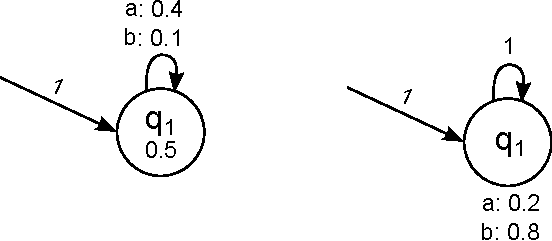
\includegraphics[scale=1]{./pictures/model-with-and-without-stop-symbols.pdf}
\label{fig:model-with-and-without-stop-symbols}
\caption{A \gls{pa} and \gls{hmm}.}
\end{centering}
\end{figure}

We will now consider the probability distributions both models define, to see what impact is has, that only the \gls{pa} defines a halting probability.
With the \gls{pa}, we can calculate the probability of generating an empty sequence, simply by starting in state 1 and stopping immediately before emitting any symbols. That is, $P_{PA}(\varepsilon) = 0.5$. We can of course also produce non empty sequences. For instance, we have that $P_{PA}(a) = \pi_1\phi_{1,a,1}F_1 = 0.2$, where $\pi_q$ is the probability of starting in state $q$, $F_q$ is the probability of stopping right after entering state $q$, $\phi_{q,s,q'}$ is the probability of going from state $q$ to state $q'$ while emitting the symbol $s$.
In the same manner, we get that $P_{PA}(b) = 0.05$.
If we in this way calculate a probability for all possible sequences, we will see that all of those probabilities sum to 1. Thus, the \gls{pa} defines a probability distribution over $\Sigma^\ast$\cite{Dupont:2005:LPA:1746577.1746601}.

When we turn our look to the \gls{hmm}, we see that its structure looks very much like the structure of a \gls{PFA]}.

Without stop probabilities, the probability definition it defines should not be interpreted in the same way as for the \gls{pa}. For instance, it does not make sense to define the probability of the empty sequence $P_{hmm}(\varepsilon)$. Also, if we start to calculate the probabilities of particular sequences in the straight forward way, we get that $P_{HMM}(a) = 0.2$, $P_{HMM}(b) = 0.8$. It is easy to see, that the missing stop probabilities causes the following property to hold:

\[\forall n, \sum_{w \in \Sigma^n} P(w) = 1\]

This means, that in contrast to the \gls{pa}, the \gls{hmm} defines a probability distribution over $\Sigma^n, \forall n \in \mathbb{N}$\cite{Dupont:2005:LPA:1746577.1746601}.

The test data of the Pautomac competation should be assigned probabilities according to a distribution over $\Sigma^\star$.
This is both stated on the Pautomac website, but could also be determined from the fact that the test set contains empty sequences. However, some small modifications allow the \gls{hmm} to behave equivalent to the \gls{pa}, in terms of defining a probability distribution over $\Sigma^\ast$. One way is to add a new symbol $x$ to $\Sigma$, which should be interpreted as a stop symbol. The symbol $x$ is then added to the end of all sequences, including the empty sequence. Instead of using a stop symbol, one could also add a single final state with no emission probabilities and no out transitions.\cite{Dupont:2005:LPA:1746577.1746601}.